%!TEX root=../../main.tex




\subsection{Galois speedup}
\label{sec:galois_speedup}
Analyzing the calculation time speedups for Galois, we can compare how or if the different algorithms benefit from increasing thread numbers.

\subsubsection{Single-source Shortest-path}
\begin{figure}
	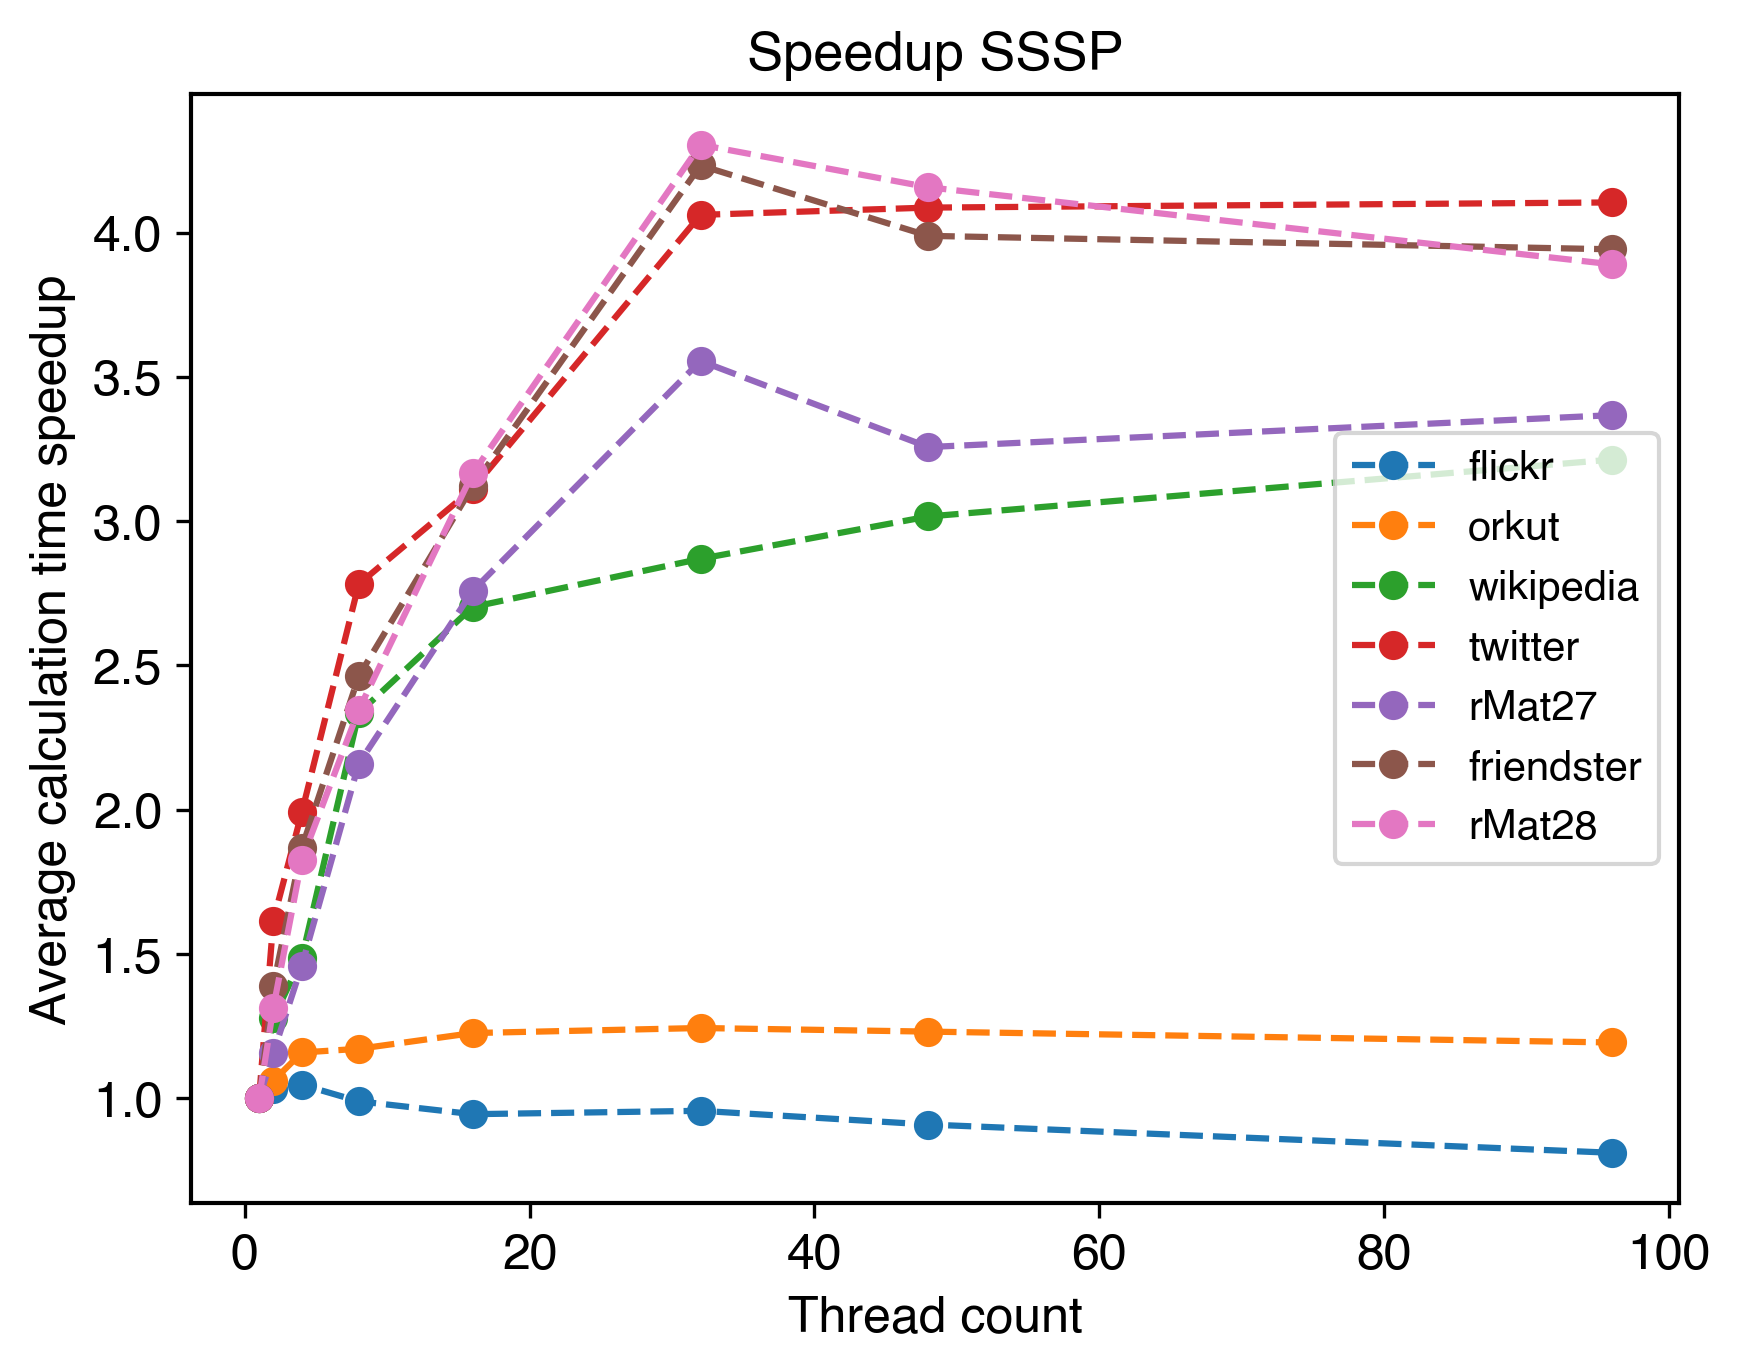
\includegraphics[width=\linewidth]{../../plots/singleNodeSSSPGaloisThreads.png}
	\caption{Calculation time speedup with increasing thread count for Galois Single-source Shortest-paths}
	\label{fig:galoisSpeedupSSSP}
\end{figure}
Starting with SSSP, we see an algorithm that benefits from many available threads in \autoref{fig:galoisSpeedupSSSP}.
For all larger graphs, speedup is in most cases very close to optimal up to about 8 threads. 
Twitter has the best speedup overall. It is 2.6$\times$ with 2 threads compared to one, 4$\times$ with 4, 7.7$\times$ with 8 and 9.7$\times$ using 16 threads.
Behaviour on friendster is similarly good. Here speedup is 1.9$\times$ at 2 threads compared to one, 3.5$\times$ at 4, 6.1$\times$ at 8 threads and 9.7$\times$ at 16 threads.
Anything above 16 threads however no longer helps decrease the computation time significantly on any graph. Speedup above 16 threads is always less than double the speedup of 16 threads. The maximum measured speedups are 10$\times$ (96 threads) for wikipedia, 17$\times$ (96 threads) for twitter, 11$\times$ (96 threads) for rMat27, 16$\times$ (48 threads) for friendster and 19$\times$ (40 threads) for rMat28.
In some cases increasing thread counts even prolongues calculation time. For example calculation on rMat28 is actually slower with 48 or 96 threads compared to 40 threads. For 40 threads, the speedup is nearly 19$\times$, on 48 threads 17$\times$ and with 96 threads only 15$\times$ compared to one thread.

Small graphs, i.e. flickr and orkut neither benefit from more threads nor is the performance significantly held up by synchronization overhead.
Performance on flickr can not be sped up at all, with speedup on flickr being very close to 1 for 1 to 8 threads and between 0.7$\times$ to 0.9$\times$ from 16 to 96 threads.
Orkut reaches maximum speedup of 1.6$\times$ at 16 threads. However on orkut, the speedup is always greater or equal to 1.



\subsubsection{Breadth-first search}
\begin{figure}
	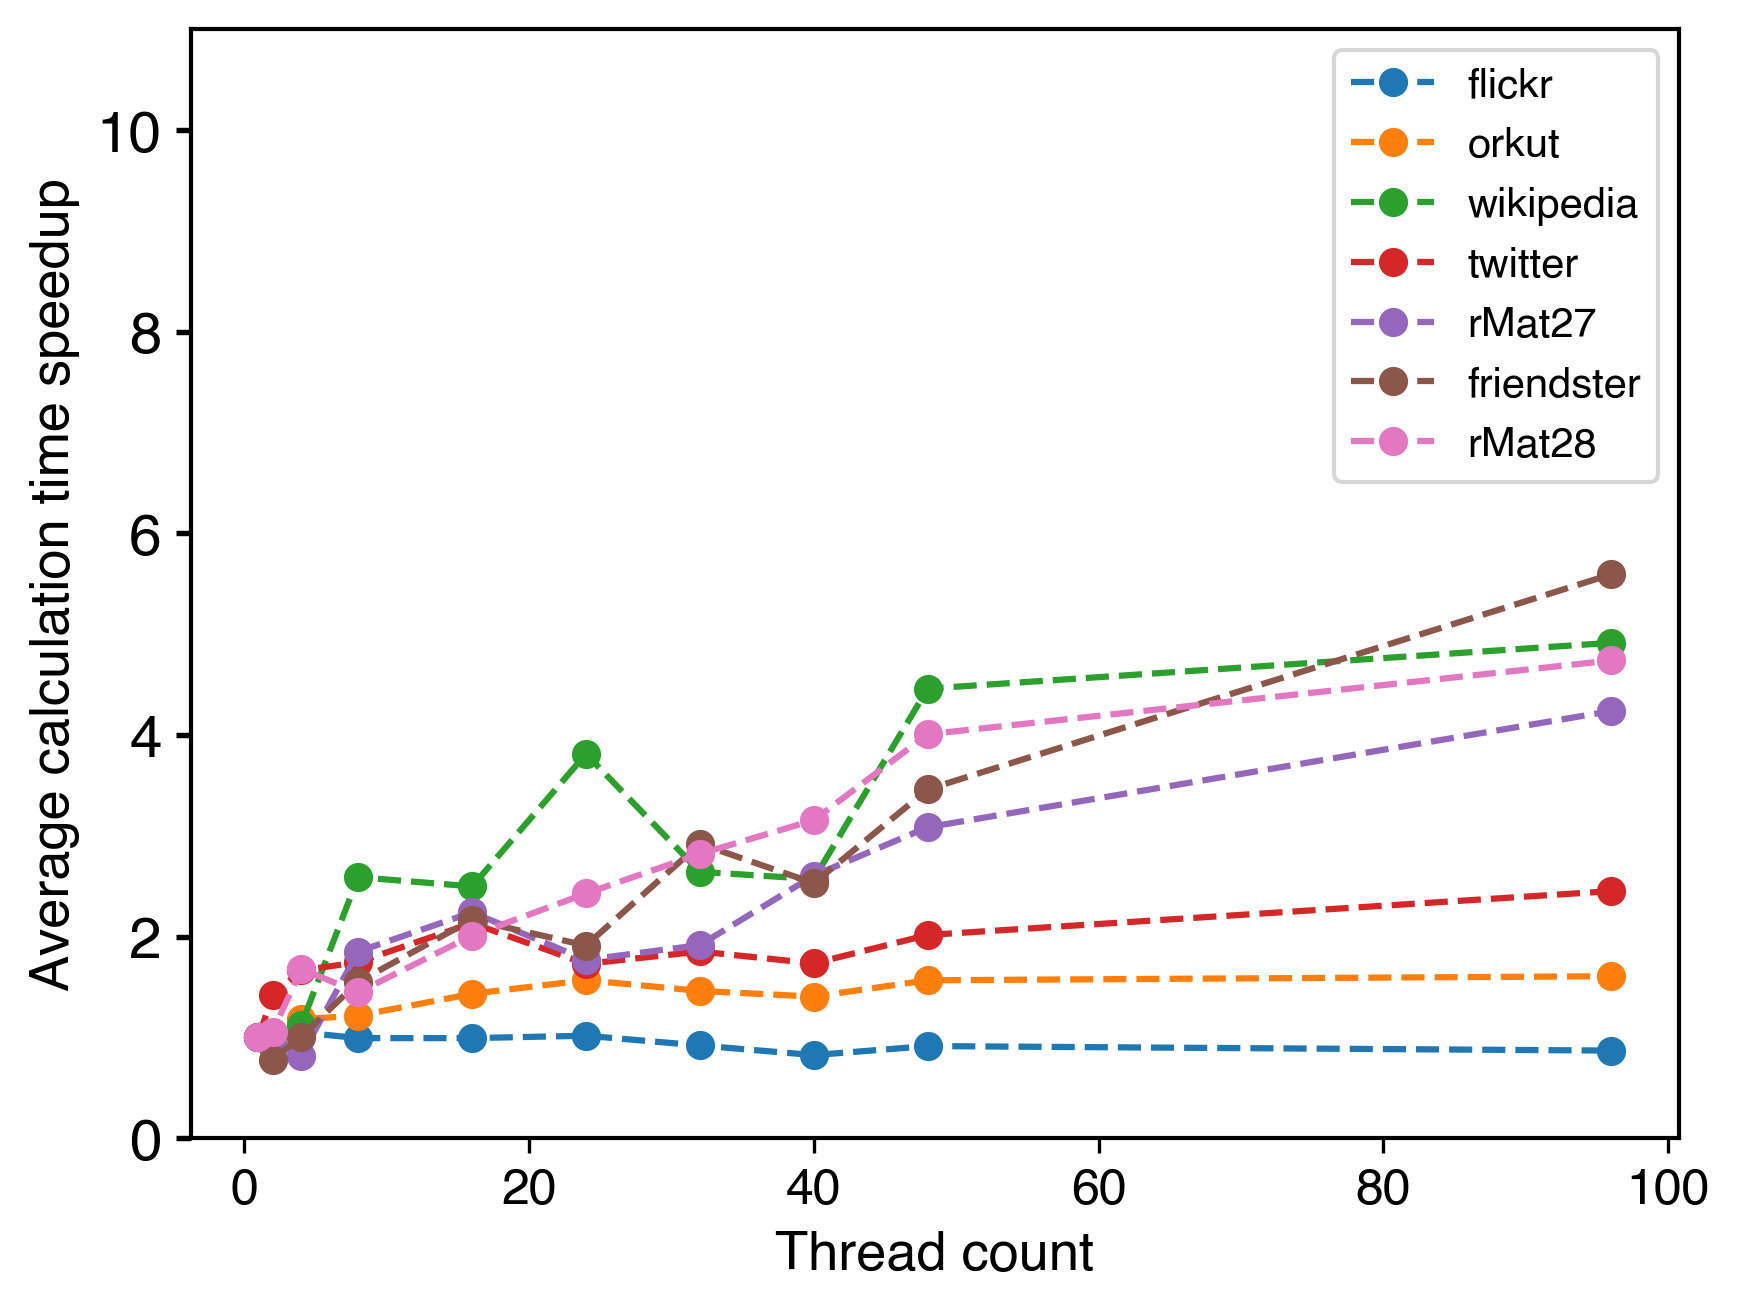
\includegraphics[width=\linewidth]{../../plots/singleNodeBFSGaloisThreads.png}
	\caption{Calculation time speedup with increasing thread count for Galois Breadth-first search}
	\label{fig:galoisSpeedupBFS}
\end{figure}

For our speedup results on BFS, \autoref{fig:galoisSpeedupBFS} shows the calculation time speedup of Galois' BFS.

Flickr is sped up by about 5\%\ with 4 threads, any more than that will actually decrease performance, making computation time up to 15\%\ (96 threads) longer.

On all graphs, the speedup never exceeds 6$\times$ even when using 96 threads.
The initial speedup when switching from one to two threads is actually smaller than one, thus decreasing performance, on 4 of 7 graphs. Only flickr, twitter and rMat28 can benefit slightly by a speedup of 2\%, 41\%\ and 5\%\ respectively.

When comparing four threads to one, BFS on all but two graphs can be sped up by anywhere from 5\%\ (flickr) to 68\% (rMat28). The speedup is thus only possible to a very small degree.
For the other two graphs, computation on friendster with 8 threads is just as fast as one thread and computation on rMat27 is actually 19\% slower.








\subsubsection{PageRank}
We want to first take a look at the results for PageRank in Pull mode, seen in \autoref{fig:galoisSpeedupPRPull}. This is a perfect example for an algorithm that does not benefit from multithreaded computation. 
Computation is hardly sped up on any graph other than flicker, where the reached maximum is 64\%. This maximum is reached at two threads, with speedup steadily declining above that.
The rMat28 is the only other graph of one could say computation was sped up. Here we reached a maximum speedup of 31\%\ at 96 threads.
All 5 other graphs only reach a speedup greater or equal to 1 in just one or two cases and if so only by a small margin.
Computation on Orkut and Twitter reaches a speedup maximum of 12\%\ and 5\%\ at 4 threads, while being less or equal to 1 in all other cases.
The wikipedia graph is never sped up.
Friendster and rMat27 can be sped up by 6.5\%\ or 10\%\ respectively on 8 threads.

Speedup results on PageRank show odd behaviour in the Galois implementation.
There is a significant performance loss on 4, 24 and 40 threads that is far from the expected behaviour. This is most visible for the Push variant seen in \autoref{fig:galoisSpeedupPRPush}, we validated the shown results two times.
Especially, the speedup for 24 threads is (by interpolating between 16 and 32 threads) expected to be anywhere between 25\% and 94\%.
Actually however, the system does not reach a speedup of more than 4\%\ on any graph, with only rMat27 actually reaching a value greater than 1. 
On all other graphs, using 24 threads is anywhere from 3\% (flickr) to 9\%\ (wikipedia) slower than using just one thread.

Similar yet less pronounced behaviour is oberservable for Pull in \autoref{fig:galoisSpeedupPRPull}. 
Here especially the values for 24 and 40 threads show a loss in performance.
It is most visible on the values for twitter and friendster, where both values drop significantly compared to the neighbouring 32 and 48 thread results.

\begin{figure}
	\begin{subfigure}{\columnwidth}
		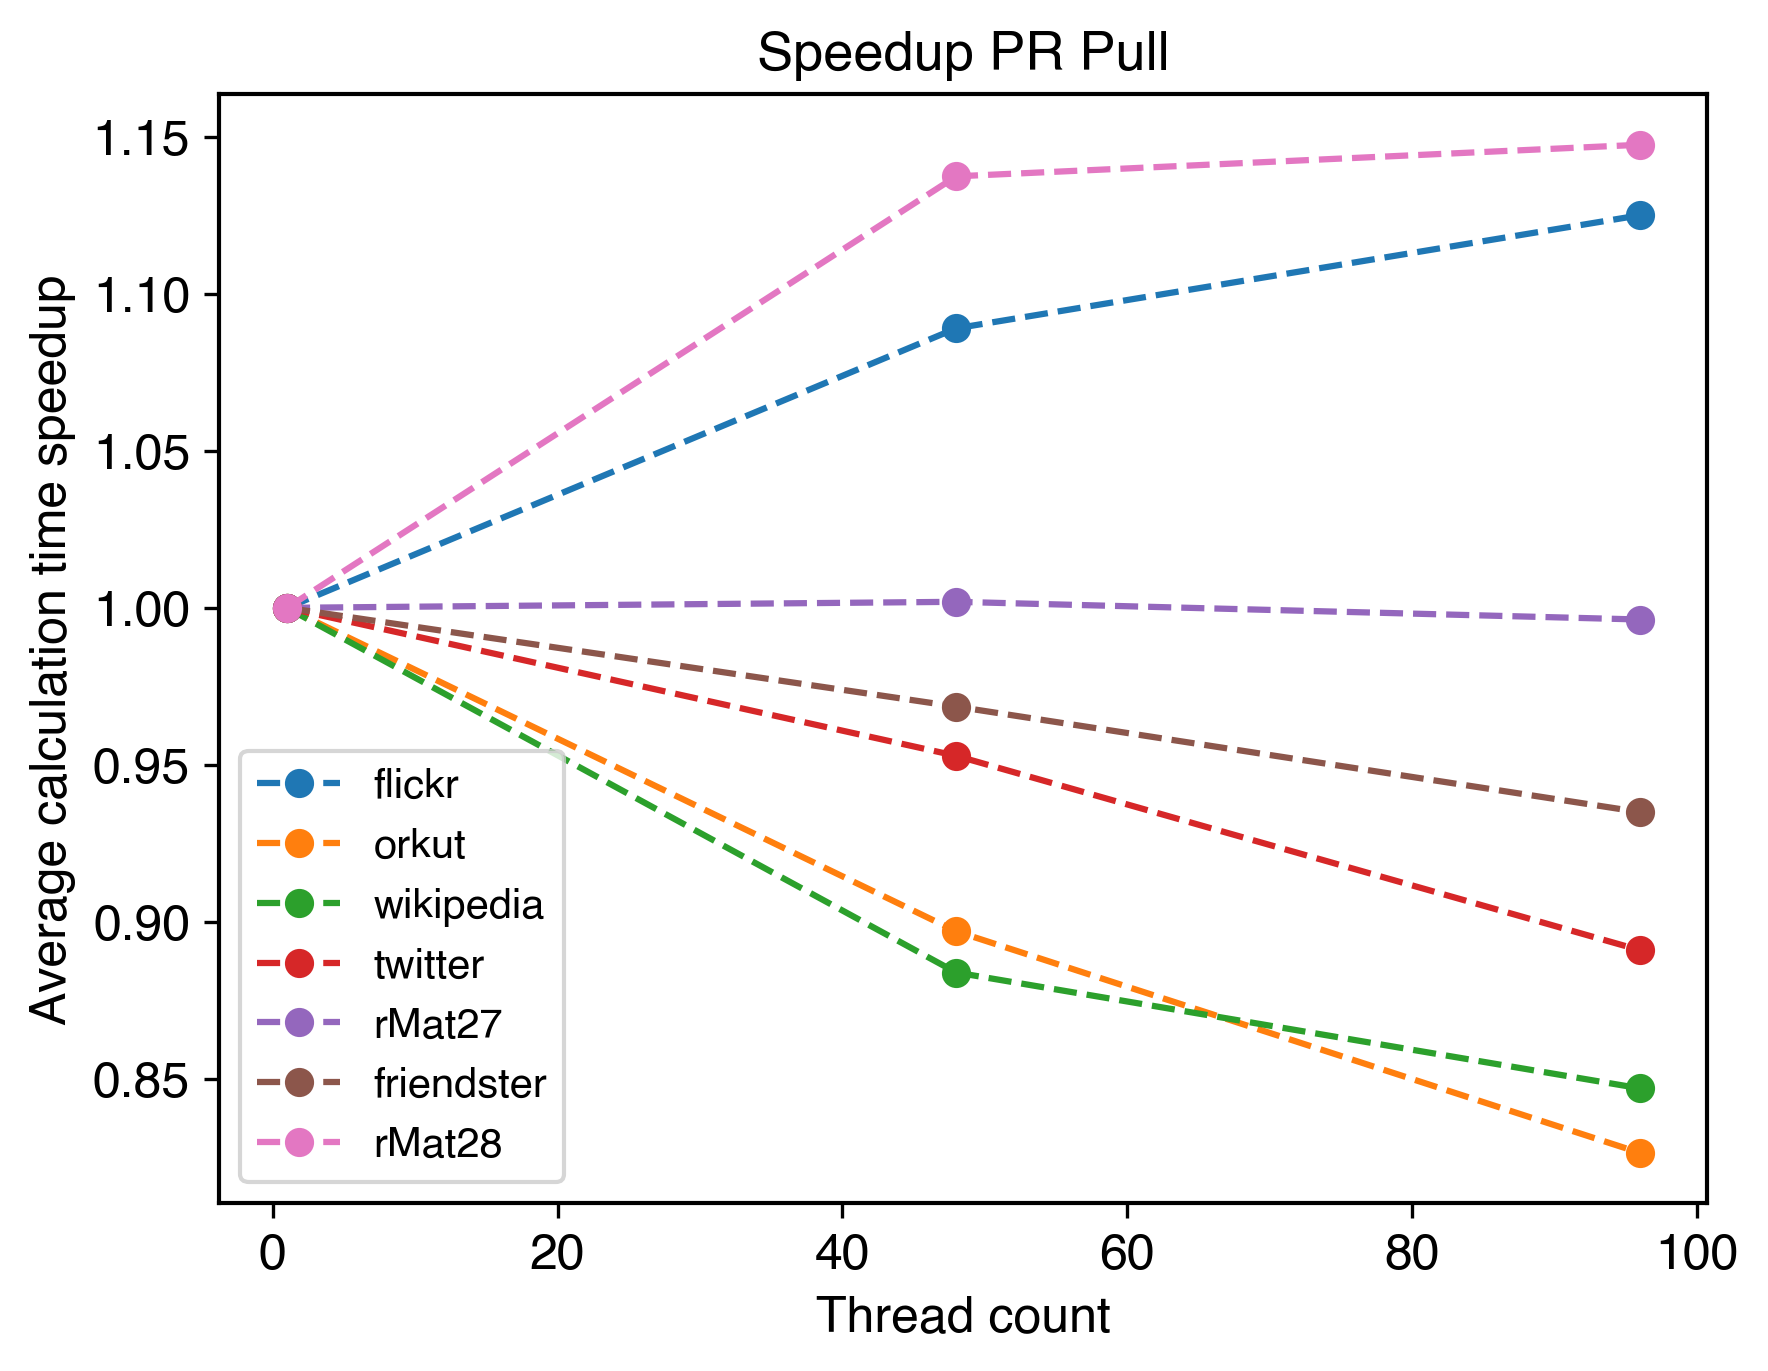
\includegraphics[width=\linewidth]{../../plots/singleNodePRPullGaloisThreads.png}
		\caption{PageRank Pull}
		\label{fig:galoisSpeedupPRPull}
	\end{subfigure}
	\begin{subfigure}{\columnwidth}
		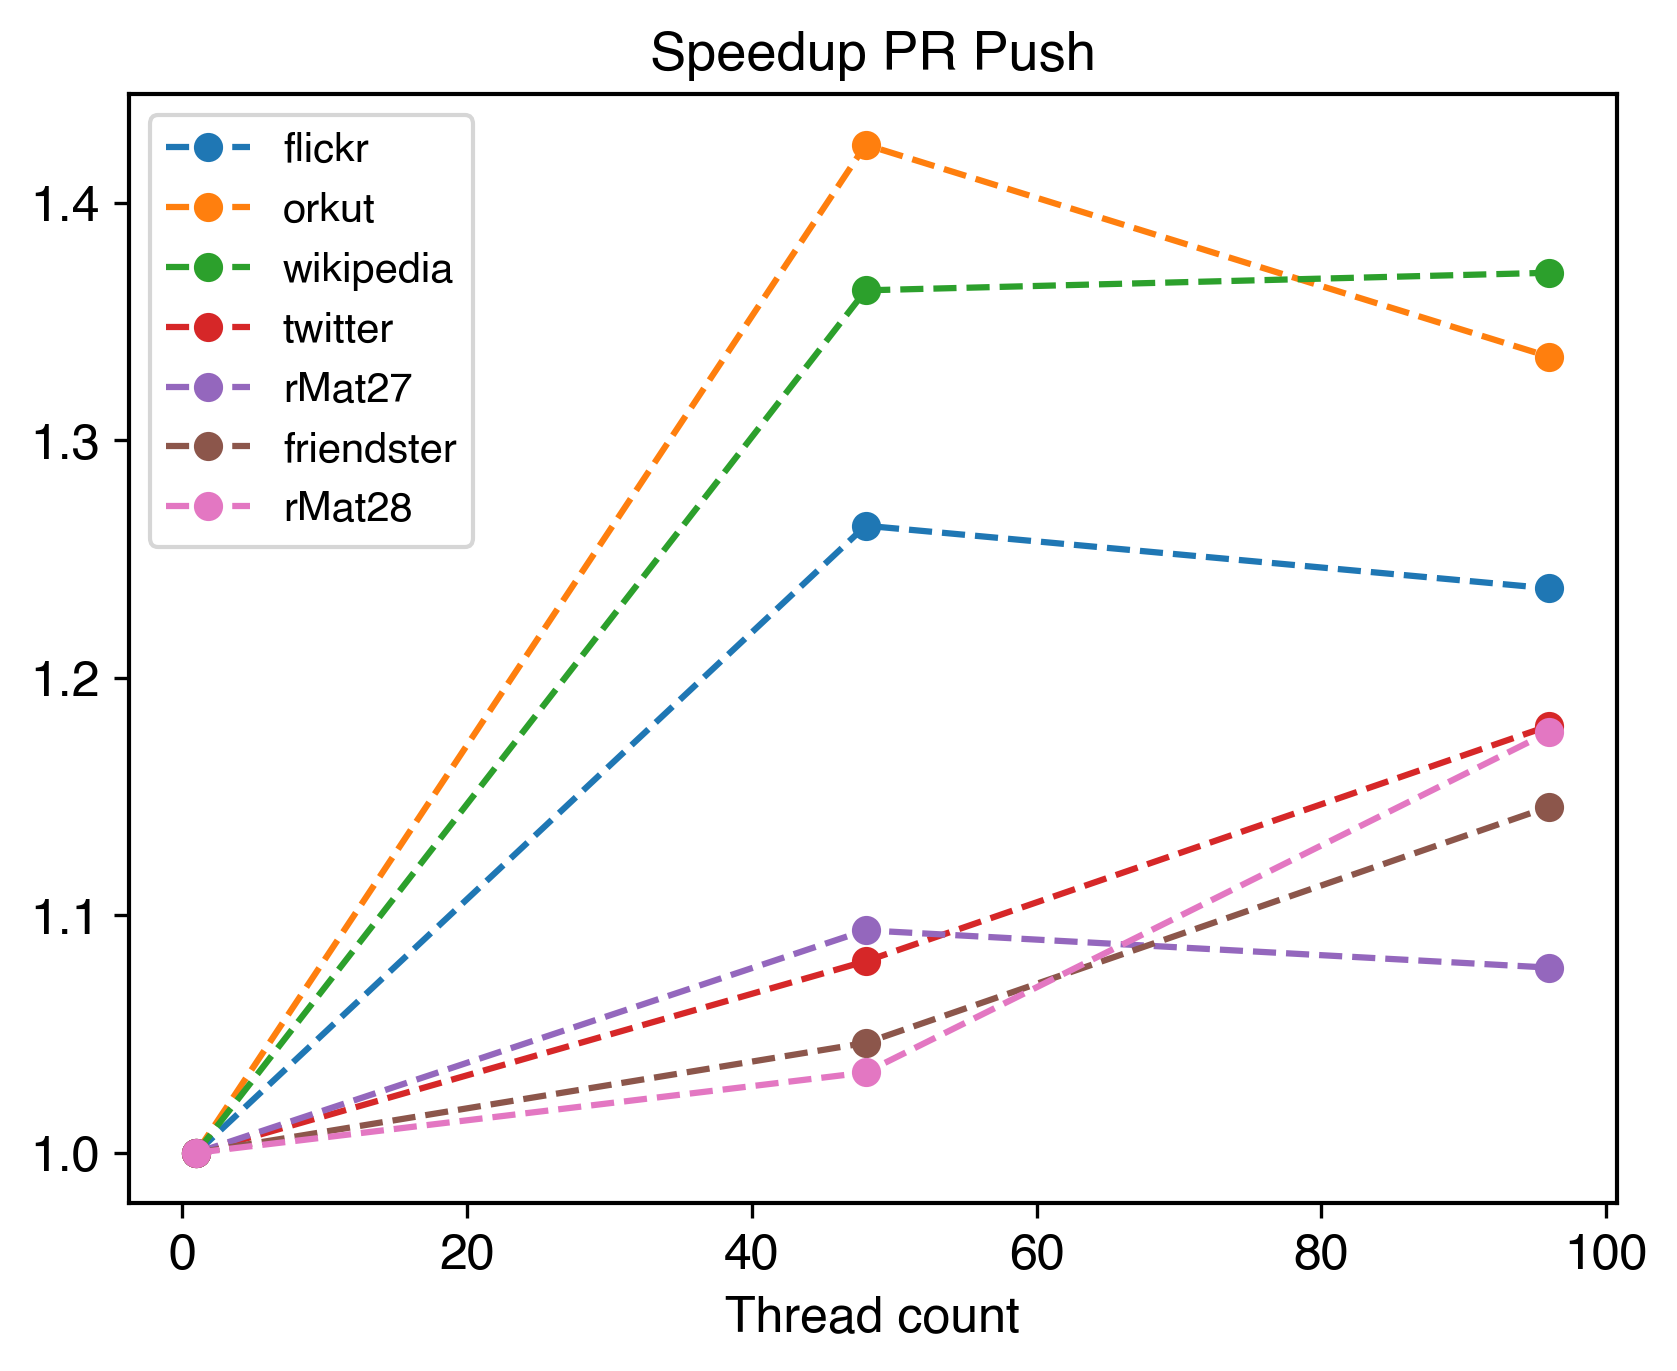
\includegraphics[width=\linewidth]{../../plots/singleNodePRPushGaloisThreads.png}
		\caption{PageRank Push}
		\label{fig:galoisSpeedupPRPush}
	\end{subfigure}
	\caption{Calculation time speedup with increasing thread count for Galois PageRank Push and Pull algorithms.}
\end{figure}


\section{Hugepages}
\begin{figure}
	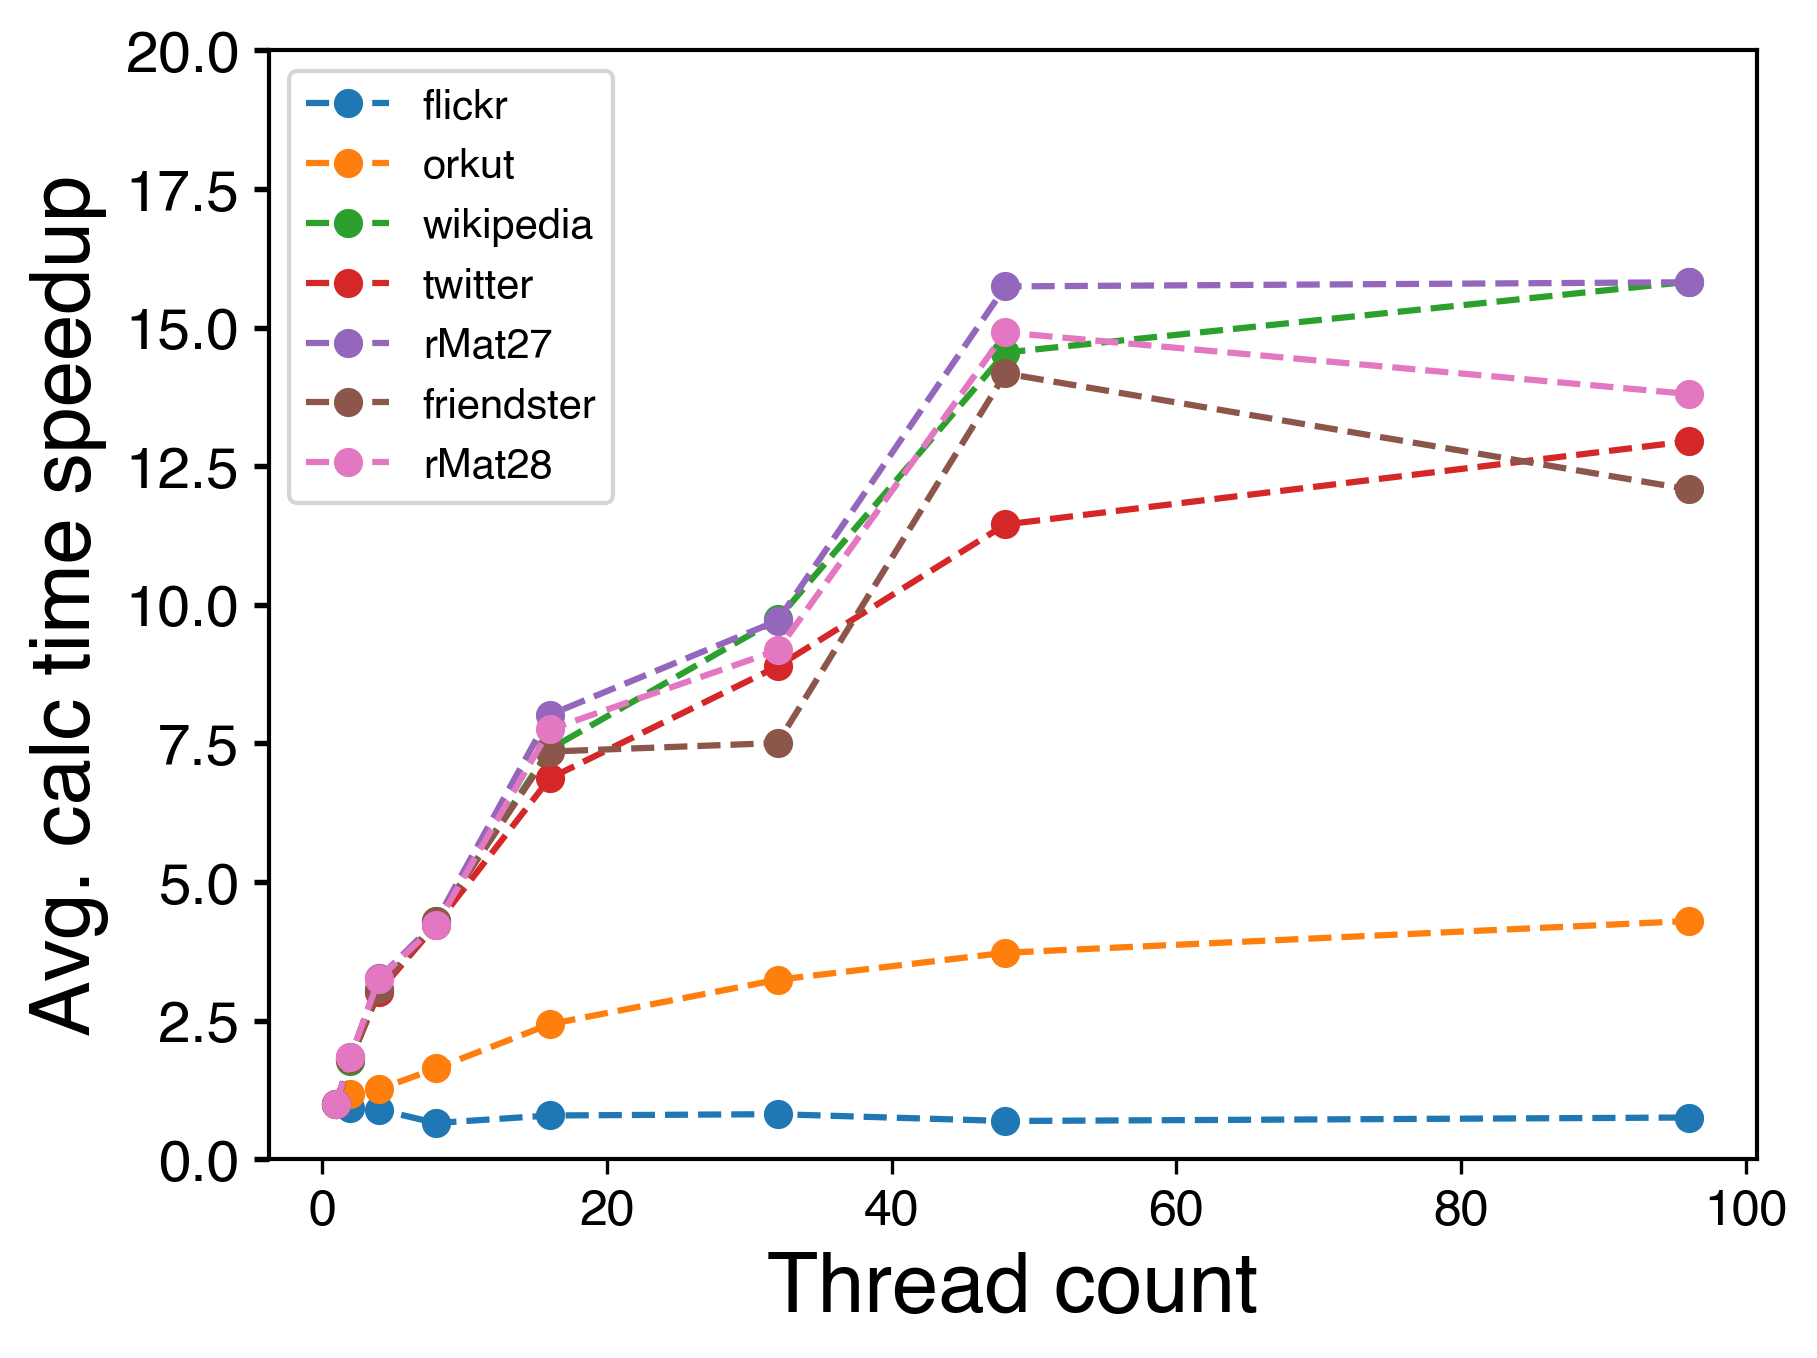
\includegraphics[width=\linewidth]{../../plots/singleNodeSSSPGaloisHPThreads.png}
	\caption{Calculation time speedup with increasing thread count for Galois Single-source Shortest-paths with Hugepages}
	\label{fig:galoisHPSpeedupSSSP}
\end{figure}

\begin{figure}
	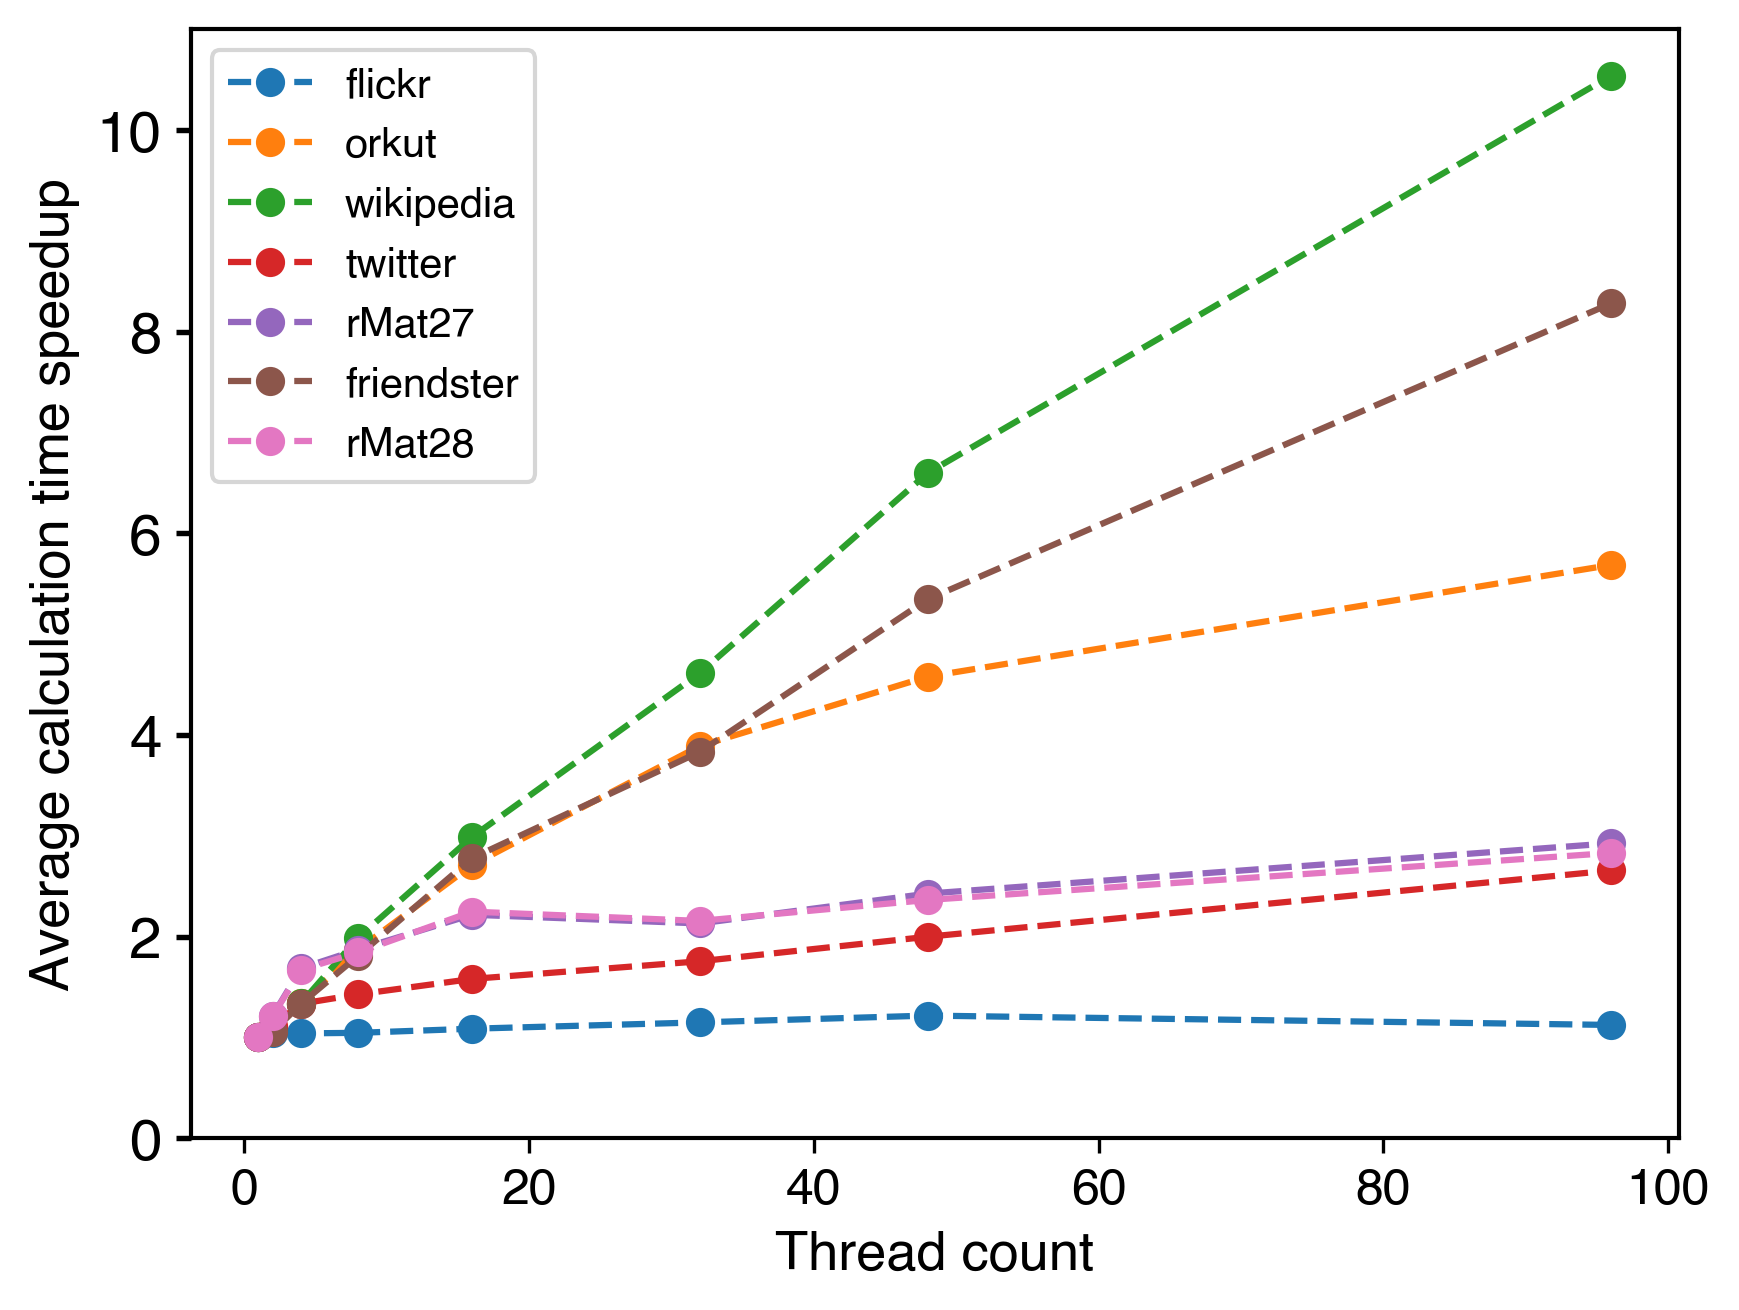
\includegraphics[width=\linewidth]{../../plots/singleNodeBFSGaloisHPThreads.png}
	\caption{Calculation time speedup with increasing thread count for Galois Breadth-first search with Hugepages}
	\label{fig:galoisHPSpeedupBFS}
\end{figure}

\begin{figure}
	\begin{subfigure}{\columnwidth}
		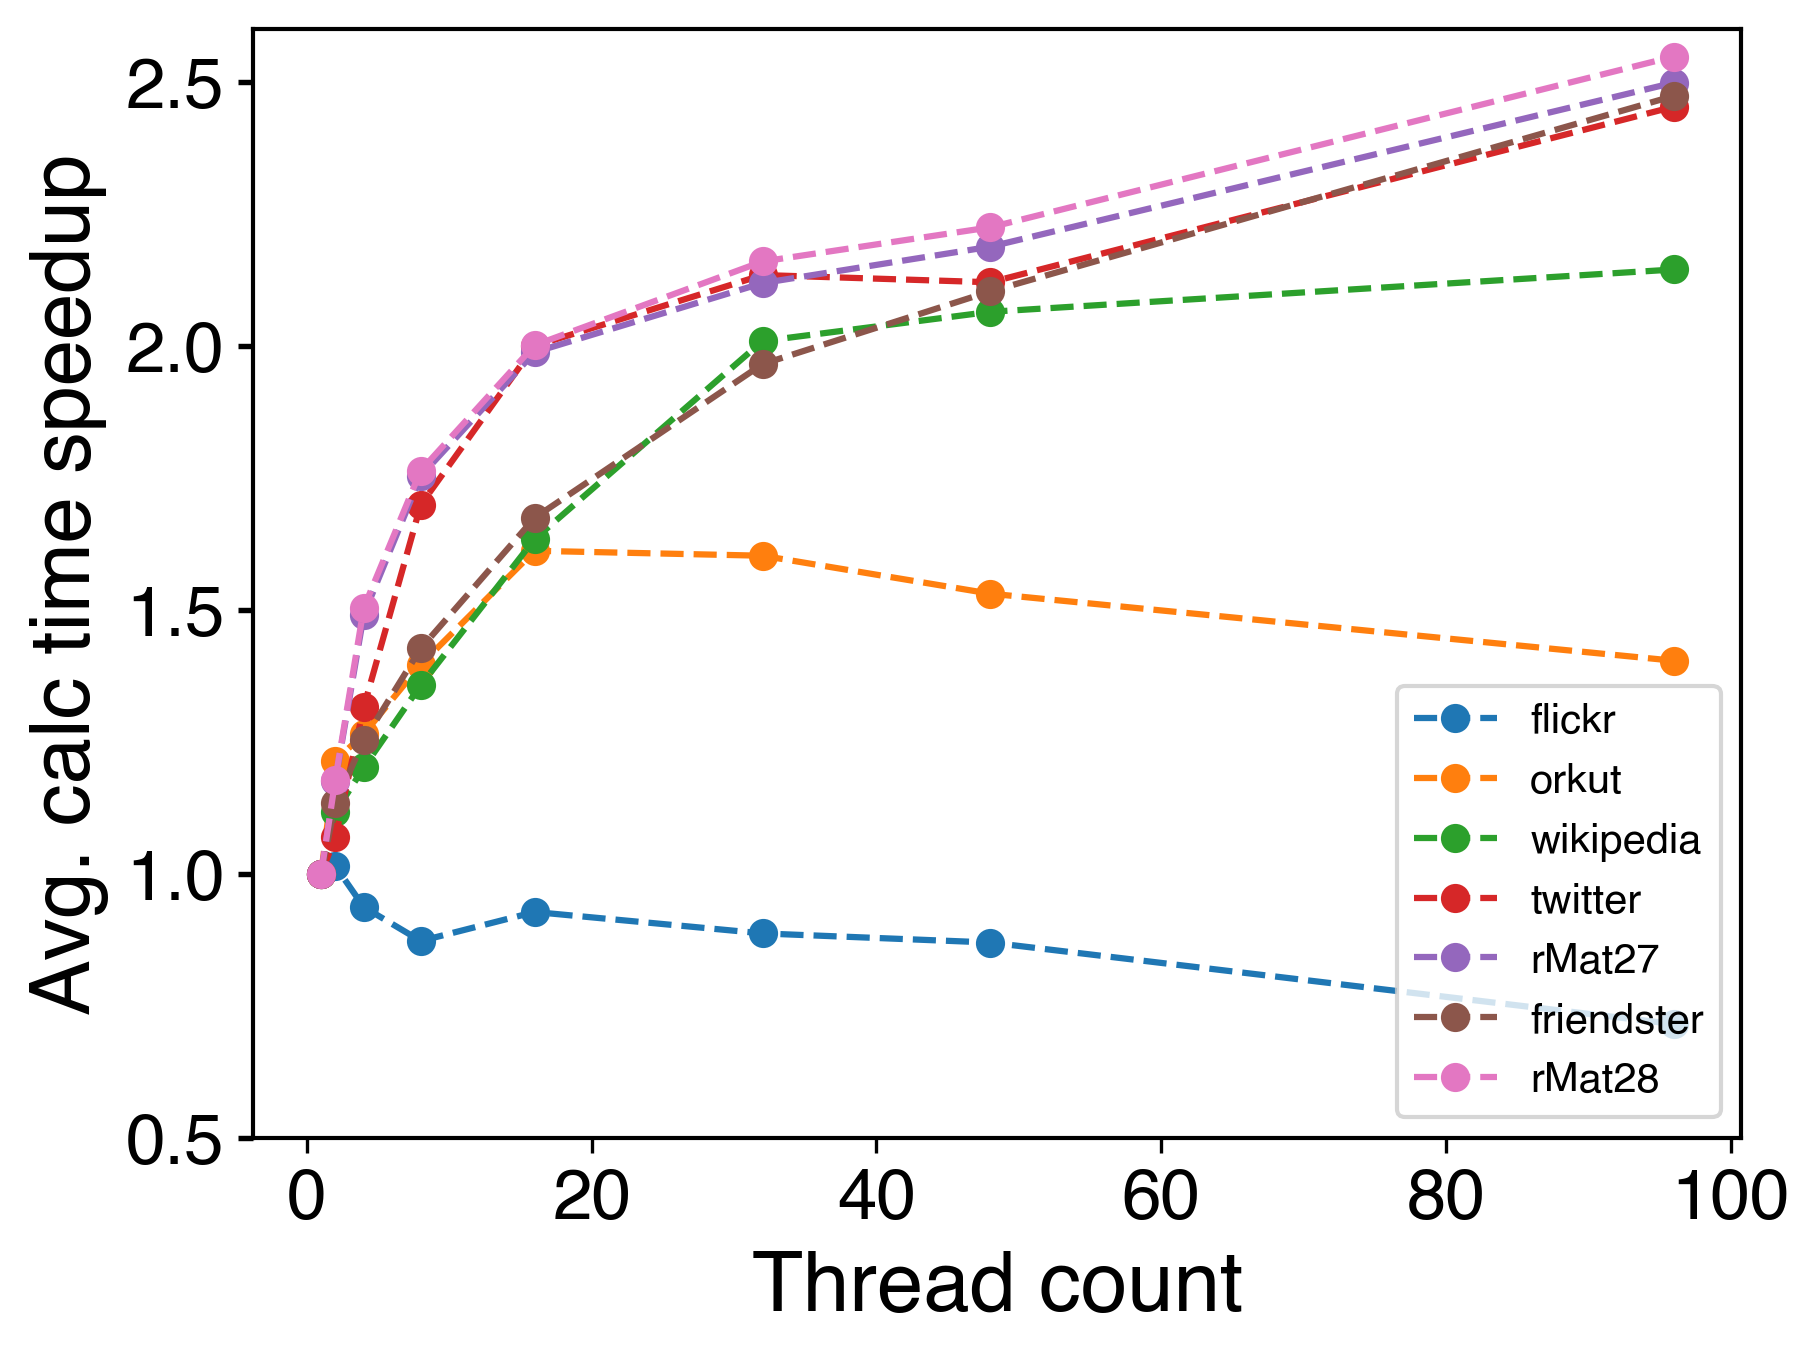
\includegraphics[width=\linewidth]{../../plots/singleNodePRPullGaloisHPThreads.png}
		\caption{PageRank Pull}
		\label{fig:galoisHPSpeedupPRPull}
	\end{subfigure}
	\begin{subfigure}{\columnwidth}
		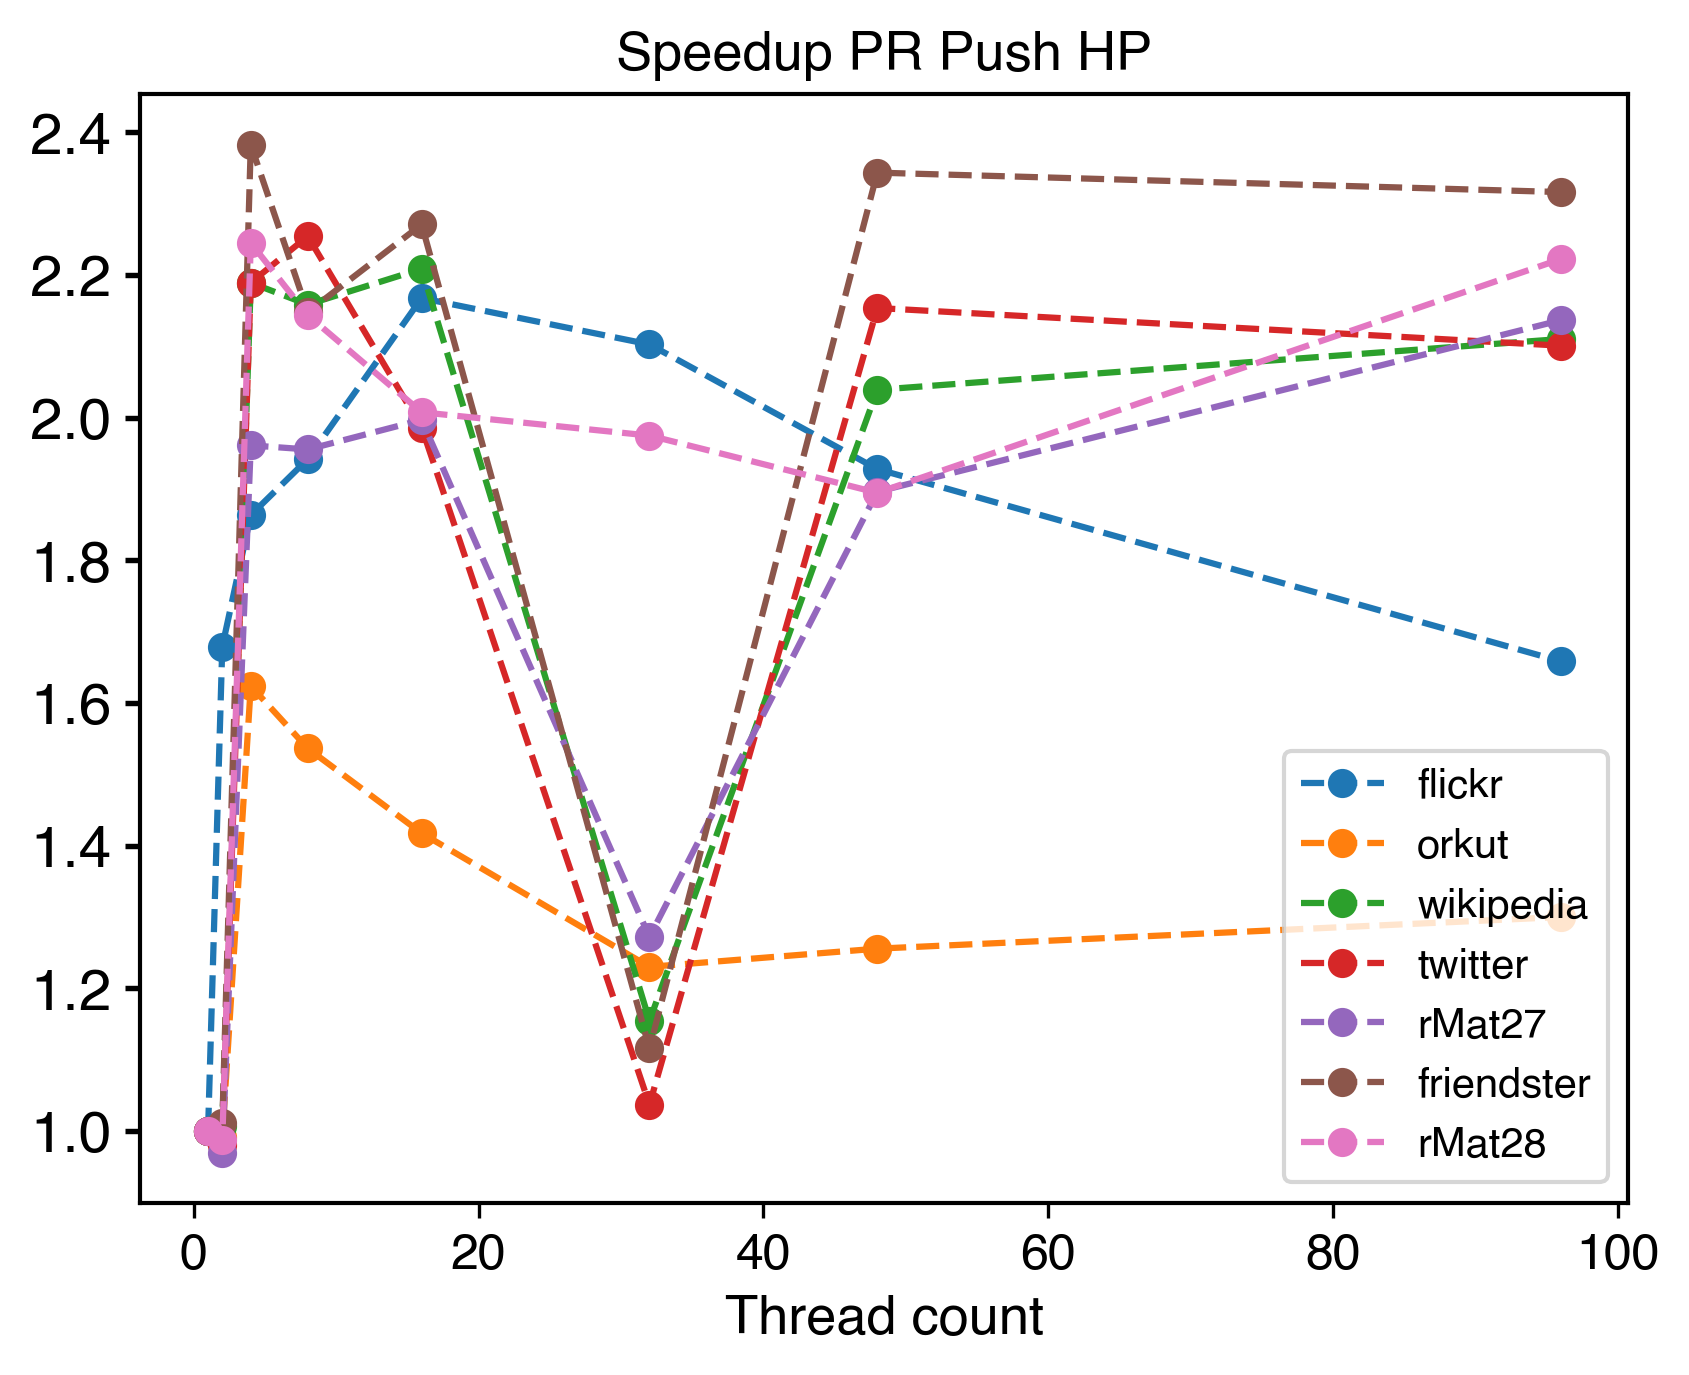
\includegraphics[width=\linewidth]{../../plots/singleNodePRPushGaloisHPThreads.png}
		\caption{PageRank Push}
		\label{fig:galoisHPSpeedupPRPush}
	\end{subfigure}
	\caption{Calculation time speedup with increasing thread count for Galois PageRank Push and Pull algorithms using Hugepages.}
\end{figure}
